\documentclass[t,8pt]{beamer}
\beamertemplatenavigationsymbolsempty

\definecolor{GitRed}{RGB}{240, 60, 46}
\setbeamercolor{title}{bg=GitRed,fg=white}
\setbeamercolor{structure}{fg=black}
\setbeamertemplate{section in toc shaded}[default][40]
\setbeamercolor{itemize item}{fg=GitRed}
\setbeamercolor{section in toc}{bg=GitRed,fg=white}
\setcounter{tocdepth}{1}
\setbeamertemplate{section in toc}{\inserttocsectionnumber.~\inserttocsection}

% Quotations
\usepackage{epigraph}
\setlength\epigraphwidth{8cm}
\setlength\epigraphrule{0pt}
\usepackage{etoolbox}
\makeatletter
\patchcmd{\epigraph}{\@epitext{#1}}{\itshape\@epitext{#1}}{}{}
\makeatother


\usepackage{url}
\usepackage{relsize}
\usepackage{hyperref}
\hypersetup{colorlinks=true, urlcolor=structure.fg, linkcolor=structure.fg}
\renewcommand*{\UrlFont}{\ttfamily\footnotesize\relax}

\usepackage{bold-extra} % cmtt
\renewcommand{\ttdefault}{cmtt}
%\usepackage{lmodern}
%\usepackage{pxfonts}  % Palatino font
%%\usepackage{txfonts}  % Times font

\makeatletter
\newcommand\handoutmode[1]{
  \ifnum1=0#1
    \gdef\beamer@currentmode{handout}
    \usepackage{../handoutWithNotes}
    \pgfpagesuselayout{4 on 1}[a4paper, landscape, border shrink=5mm]
    \setbeamertemplate{navigation symbols}{}
    \setbeamertemplate{headline}{%
      \leavevmode%
      \vspace{.5cm}
    }



    % define font of lstlisting
    \lstset{
      basicstyle=\ttfamily\bfseries, %\tiny\ttfamily,
      tabsize=2,
      extendedchars=true,
      breaklines=true,
      %frame=single,
      %stringstyle=\ttfamily,
      showspaces=false,
      showtabs=false,
      xleftmargin=.25cm,
      %framextopmargin=0pt,
      %framexleftmargin=2pt,
      %framexrightmargin=2pt,
      %framexbottommargin=0pt,
      backgroundcolor=\color{white},
      showstringspaces=false
      %morestring=[b][\color{blue}]",
      %morestring=[d][\color{blue}]',
      columns=fullflexible,
      escapeinside={(*}{*)},
      keepspaces=true,
      upquote=true,
      commentstyle=\color{red},
      keywordstyle=\color{blue},
      rulecolor=\color{gray}
    %  language=bash
    }
    %\lstloadlanguages{bash}
  \else
    \AtBeginSection[]{
      \begin{frame}<*>{Outline}
        \hspace{1.2em}
        \begin{multicols}{2}
        \frametitle{Outline}
        \tableofcontents[currentsection] %,hideallsubsections]
        \end{multicols}
      \end{frame}
    }
    \addtocontents{toc}{\vskip -0.2cm}
    \setbeamertemplate{footline}[text line]{%
      \parbox{\linewidth}{\vspace*{-8pt}\textcolor{lightgray}{\inserttitle{} {\normalsize\ttfamily\textcopyright}\ \insertauthor\ \the\year \hfill \insertpagenumber/\pageref{LastPage}}}
    }
    \setbeamertemplate{navigation symbols}{}

    \setbeamercolor{title}{fg=white, bg=GitRed}
    \setbeamercolor{frametitle}{fg=white, bg=GitRed}

    \setbeamercolor{section in toc}{fg=black,bg=white}

    \setbeamertemplate{frametitle}
    {
        \nointerlineskip
        \begin{beamercolorbox}[sep=0.01cm,ht=1.8em,wd=\paperwidth]{frametitle}
          %\vbox{}\vskip-4ex%
          \hspace{.3cm}\strut\textbf\insertframetitle\strut
          %\vskip-0.8ex%
          \hfill$\vcenter{\hbox{\includegraphics{diagrams/git-logo-small.pdf}}}$
        \end{beamercolorbox}
    }

    % define font of lstlisting
    \definecolor{listingbackground}{rgb}{0,0,0}
    \lstset{
      basicstyle=\ttfamily\bfseries\color{black}, %\tiny\ttfamily,
      tabsize=2,
      extendedchars=true,
      breaklines=true,
      frame=leftline,
      %stringstyle=\ttfamily,
      showspaces=false,
      showtabs=false,
      xleftmargin=.25cm,
      %framextopmargin=0pt,
      %framexleftmargin=2pt,
      %framexrightmargin=2pt,
      %framexbottommargin=0pt,
      backgroundcolor=\color{white},
      showstringspaces=false
      %morestring=[b][\color{blue}]",
      %morestring=[d][\color{blue}]',
      columns=fullflexible,
      escapeinside={(*}{*)},
      keepspaces=true,
      upquote=true,
      commentstyle=\color{red},
      keywordstyle=\color{blue},
      rulecolor=\color{gray}
    %  language=bash
    }
    %\lstloadlanguages{bash}

  \fi
}
\makeatother

\usepackage{catchfile}
\newcommand{\getenv}[2][]{%
  \CatchFileEdef{\temp}{"|kpsewhich --var-value #2"}{}%
  \if\relax\detokenize{#1}\relax\temp\else\let#1\temp\fi}

\usepackage{listings}

\getenv[\HANDOUT]{HANDOUT}
\handoutmode{\HANDOUT}

\usepackage[utf8]{inputenc}
\usepackage{multicol}
\usepackage{color,soul}
\usepackage{tabto}
\usepackage{inconsolata}
\usepackage{graphicx}
\usepackage{wrapfig}
\usepackage{upquote}
\usepackage{vwcol}
\usepackage{lastpage}

% table spacings
\renewcommand{\arraystretch}{1.5}

%\setlength{\parskip}{10pt plus 1pt minus 1pt}

\newcommand{\slidetitle}{\frametitle{\thesection. \secname}\vspace{1em}}
\newcommand{\subslidetitle}{\frametitle{\thesection.\thesubsection\ \subsecname}\vspace{1em}}
\newcommand{\subsubslidetitle}{\frametitle{\thesection.\thesubsection.\thesubsubsection\ \subsubsecname}\vspace{1em}}

\newcommand{\cmd}[1]{\textcolor[HTML]{0000AA}{\texttt{\textbf{#1}}}}
\newcommand{\option}[3][1cm]{\item[]{\usebeamercolor[structure.fg]{section in head}\texttt{#2}}\tabto{#1}#3}

\def\braces#1{[#1]}
\def\lbrace#1{[#1}

\newcounter{exercise}
\newenvironment{exercise}[0]
  {\begin{enumerate}\setcounter{enumi}{\theexercise}}
  { \setcounter{exercise}{\theenumi}\end{enumerate}}

% layout of title side
\makeatletter
\setbeamertemplate{title page}
{
  \vspace{.6cm}
  \center \includegraphics{diagrams/git-logo-2color.pdf}
  \vbox{}
  \vfill
  \begingroup
    \centering
    \begin{beamercolorbox}[sep=8pt,center]{title}
      \usebeamerfont{title}\bf{\Huge{workshop}}\par%
      \ifx\insertsubtitle\@empty%
      \else%
        \vskip0.25em%
        {\usebeamerfont{subtitle}\usebeamercolor[fg]{subtitle}\insertsubtitle\par}%
      \fi%
    \end{beamercolorbox}%
    \vskip1em\par
    \begin{beamercolorbox}[sep=8pt,center]{author}
      \usebeamerfont{author}\insertauthor
    \end{beamercolorbox}
    \begin{beamercolorbox}[sep=8pt,center]{institute}
      \usebeamerfont{institute}\insertinstitute
    \end{beamercolorbox}
    \begin{beamercolorbox}[sep=8pt,center]{date}
      \usebeamerfont{date}\insertdate
    \end{beamercolorbox}\vskip0.5em
  \endgroup
  \vfill
}
\makeatother
% end of layout of title side

\begin{document}
\title{git workshop}
\author{André Roth, Andreas Schmid, Eric Keller}

\date{\today}


\frame{\titlepage}

\section{Preface}
\begin{frame}
  \slidetitle

  Required skills:
  \begin{itemize}
    \item basic command line knowledge
    \item file editor
  \end{itemize}
  \vspace{1em}
  This workshop takes about 4 hours.
\end{frame}

\subsection{Version Control Systems}
\begin{frame}
  \subslidetitle


  \begin{tabular}{lp{5cm}}
    \textbf{1982} & Revision Control System (RCS) \\
    \pause
    \textbf{1990} & Concurrent Versions System (CVS)\\
    \pause
    \textbf{1992} & Rational ClearCase\\
    \pause
    \textbf{1995} & Perforce \\
    \pause
    \textbf{2000} & BitKeeper\\
    \pause
    \textbf{2000} & Apache Subversion (SVN) \\
    \pause
    \textbf{2005} & git \\
    \pause
    \textbf{2005} & GNU Bazaar\\
    \pause
    \textbf{2005} & Mercurial \\
    \pause
  \end{tabular}
\end{frame}

\subsection{Version Control Systems}
\begin{frame}
  \subslidetitle
  \epigraph{``Because my hatred of CVS has meant that I see Subversion as being the most pointless project ever started, because the whole slogan for the Subversion for a while was 'CVS done right' or something like that. And if you start with that kind of slogan, there is nowhere you can go. It's like, there is no way to do CVS right."}
  {--- Linus Torvalds on git, Tech Talk 200705\footnote{https://www.youtube.com/watch?v=4XpnKHJAok8}}
\end{frame}

%\subsection{Course goal}
%\frame{
  %\subslidetitle

  %This course aims to provide knowledge about:
  %\begin{itemize}
    %\item Setup git (gitconfig, alias)
    %\item Clone repository (clone)
    %\item Create local changes (status, add, commit, reset, diff, log, reflog)
    %\item Work with different branches (branch, checkout, stash, diff, rebase, merge, cherry-pick)
    %\item Work with remotes (remote, fetch, pull, push, upstream, blame)
    %\item Master merge conflict (mergetool, 3 way merge)
    %\item format-patch
    %\item Find the bug with git bisect
    %\item pull requests
    %\item Advanced git: porcelain and plumbing
  %\end{itemize}
  %\vspace{1em}
%}

%\subsection{Git workflow}
%\frame{
  %\subslidetitle

  %\begin{itemize}
    %\item Fetch or clone a repository
    %\item Modify the local files
    %\item Stage the files
    %\item Commit the changes locally
    %\item Push changes to remote repository
  %\end{itemize}
  %\vspace{1em}
%}

\section{Getting started}
\begin{frame}[fragile]
  \slidetitle

  This section covers the following topics:
  \begin{itemize}
    \pause
    \item Configure git
    \pause
    \item Obtain a git repository
    \pause
    \item Add files
    \pause
    \item Stage changes
    \pause
    \item Commit changes
    \pause
    \item The git work flow
    \pause
    \item Undo modifications and staging
  \end{itemize}
\end{frame}

\subsection{Configuring git}
\begin{frame}[fragile]
  \subslidetitle
  Many useful features can be configured with git:
  \begin{itemize}
    \item User settings
    \item Colored output
    \item Command aliases
    \item Tools to be used
  \end{itemize}

  \vspace{1em}
  The minimum configuration needs your name and email address.\\
  Let's configure this by using the \cmd{git config} command:
  \begin{lstlisting}
$ (*\textcolor[HTML]{0000AA}{git config --global user.name "My name"}*)
$ (*\textcolor[HTML]{0000AA}{git config --global user.email "myemail@address"}*)
\end{lstlisting}

  \vspace{1em}
  Note: The global git configuration is stored in \cmd{\textasciitilde/.gitconfig}.

\end{frame}

\subsection{Obtaining a repository}
\begin{frame}[fragile]
  \subslidetitle
  A git repository can be obtained only by downloading a whole git repository,
  called a working copy.
  \\
  \vspace{1em}
  Let's clone the gitmoon repository by using \cmd{git clone}:
  \begin{lstlisting}
$ (*\textcolor[HTML]{0000AA}{git clone https://github.com/neolynx/gitmoon.git}*)
Cloning into 'gitmoon'...
remote: Counting objects: 6, done.
remote: Compressing objects: 100% (6/6), done.
remote: Total 6 (delta 0), reused 6 (delta 0), pack-reused 0
Unpacking objects: 100% (6/6), done.
Checking connectivity... done.
\end{lstlisting}

  \vspace{1em}
  Note: a new repository can be created with the \cmd{git init} command.
\end{frame}

\subsection{Workshop git project}
\begin{frame}[fragile]
  \subslidetitle
  Let's see what we find in the working copy:
  \begin{lstlisting}
$ (*\textcolor[HTML]{0000AA}{cd gitmoon}*)
$ (*\textcolor[HTML]{0000AA}{ls}*)
moon_1024.jpg  moon.html  moon.js  three.min.js
\end{lstlisting}

  \vspace{1em}
  Oh, there is a HTML file !
  \begin{lstlisting}
$ (*\textcolor[HTML]{0000AA}{firefox moon.html \&}*)
\end{lstlisting}
\end{frame}

\subsection{Checking the status}
\begin{frame}[fragile]
  \subslidetitle

  The command \cmd{git status} shows the state of the local working copy:
  \begin{lstlisting}
$ (*\textcolor[HTML]{0000AA}{git status}*)
On branch master
Your branch is up-to-date with 'origin/master'.
nothing to commit, working directory clean
\end{lstlisting}
\end{frame}


\subsection{Adding a file}
\begin{frame}[fragile]
  \subslidetitle

  Let's create an AUTHORS file with your name:
  \begin{lstlisting}
$ (*\textcolor[HTML]{0000AA}{echo Tux Penguin > AUTHORS}*)
\end{lstlisting}

  Check the git status:
  \begin{lstlisting}
$ (*\textcolor[HTML]{0000AA}{git status}*)
On branch master
Your branch is up-to-date with 'origin/master'.
Untracked files:
  (use "git add <file>..." to include in what will be committed)

        (*\textcolor[HTML]{AA0000}{AUTHORS}*)

nothing added to commit but untracked files present (use "git add" to track)
\end{lstlisting}

\end{frame}

\subsection{Adding a file}
\begin{frame}[fragile]
  \subslidetitle

  The command \cmd{git add} tells git to track the file:
  \begin{lstlisting}
$ (*\textcolor[HTML]{0000AA}{git add AUTHORS}*)
\end{lstlisting}

  Check the git status:
  \begin{lstlisting}
$ (*\textcolor[HTML]{0000AA}{git status}*)
On branch master
Your branch is up-to-date with 'origin/master'.
Changes to be committed:
  (use "git reset HEAD <file>..." to unstage)

        (*\textcolor[HTML]{00AA00}{new file:}*)   (*\textcolor[HTML]{00AA00}{AUTHORS}*)
\end{lstlisting}

  \vspace{1em}
  Note: only files can be tracked, git treats directories as part of the file name
\end{frame}


\subsection{Creating a commit}
\begin{frame}[fragile]
  \subslidetitle

  The command \cmd{git commit} tells git to commit the file:
  \begin{lstlisting}
$ (*\textcolor[HTML]{0000AA}{git commit -m "add authors file"}*)

[master c01af7f] add authors file
 1 file changed, 1 insertion(+)
 create mode 100644 AUTHORS
\end{lstlisting}

  Check the git status:
  \begin{lstlisting}
$ (*\textcolor[HTML]{0000AA}{git status}*)
On branch master
Your branch is ahead of 'origin/master' by 1 commit.
  (use "git push" to publish your local commits)
nothing to commit, working directory clean
\end{lstlisting}
\end{frame}

\subsection{Git workflow}
\begin{frame}[fragile]
  \subslidetitle
  The following diagram illustrates the workflow we just did: \\
  \vspace{2em}
  \centerline{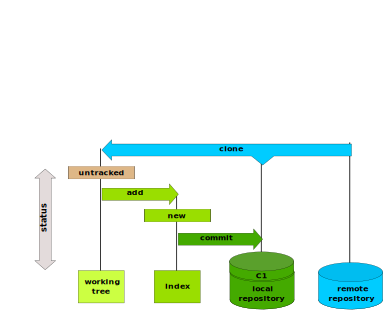
\includegraphics{diagrams/getting_started.pdf}}

  \vspace{1em}
  Note: the \textbf{index} is also called \textbf{staging area}
\end{frame}


\subsection{Modifying a file}
\begin{frame}[fragile]
  \subslidetitle

  Let's change the \cmd{<title>} tag of \cmd{moon.html} to 'Git Moons':
  \begin{lstlisting}
$ (*\textcolor[HTML]{0000AA}{vi moon.html}*)
\end{lstlisting}

  Check the git status:
  \begin{lstlisting}
$ (*\textcolor[HTML]{0000AA}{git status}*)
On branch master
Your branch is up-to-date with 'origin/master'.
Changes not staged for commit:
  (use "git add <file>..." to update what will be committed)
  (use "git checkout -- <file>..." to discard changes in working directory)

        (*\textcolor[HTML]{AA0000}{modified:}*)   (*\textcolor[HTML]{AA0000}{moon.html}*)

no changes added to commit (use "git add" and/or "git commit -a")
\end{lstlisting}
\end{frame}

\subsection{Showing changes}
\begin{frame}[fragile]
  \subslidetitle

  The command \cmd{git diff} show the difference between working tree and index:
  \begin{lstlisting}
$ (*\textcolor[HTML]{0000AA}{git diff}*)
diff --git a/moon.html b/moon.html
index d344c62..22e0c8e 100644
--- a/moon.html
+++ b/moon.html
(*\textcolor[HTML]{0000EE}{@@ -1,7 +1,7 @@}*)
 <!DOCTYPE html>
 <html>
     <head>
(*\textcolor[HTML]{AA0000}{-}*)        (*\textcolor[HTML]{AA0000}{<title>moon</title>}*)
(*\textcolor[HTML]{00AA00}{+}*)        (*\textcolor[HTML]{00AA00}{<title>Git Moons</title>}*)
         <meta charset="utf-8">
\end{lstlisting}
\end{frame}

\subsection{Staging modifications}
\begin{frame}[fragile]
  \subslidetitle

  The command \cmd{git add} tells git to stage the modifications:
  \begin{lstlisting}
$ (*\textcolor[HTML]{0000AA}{git add moon.html}*)
\end{lstlisting}

  Check the git status:
  \begin{lstlisting}
$ (*\textcolor[HTML]{0000AA}{git status}*)
On branch master
Your branch is up-to-date with 'origin/master'.
Changes to be committed:
  (use "git reset HEAD <file>..." to unstage)

        (*\textcolor[HTML]{00AA00}{modified:}*)   (*\textcolor[HTML]{00AA00}{moon.html}*)
\end{lstlisting}
\end{frame}

\subsection{Committing staged changes}
\begin{frame}[fragile]
  \subslidetitle

  The command \cmd{git commit} tells git to commit the index to the local repository:
  \begin{lstlisting}
$ (*\textcolor[HTML]{0000AA}{git commit -m "change title"}*)
[master fc92204] change title
 1 file changed, 1 insertion(+), 1 deletion(-)
\end{lstlisting}
\end{frame}

\subsection{Git workflow}
\begin{frame}[fragile]
  \subslidetitle
  The following diagram illustrates the workflow we just did: \\
  \vspace{2em}
  \centerline{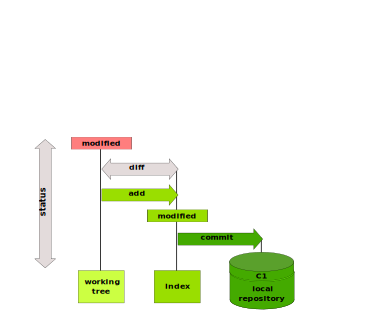
\includegraphics{diagrams/diff-modified-add-commit.pdf}}
\end{frame}

\subsection{Undoing a modification}
\begin{frame}[fragile]
\subslidetitle

  Let's modify a file and verify the git status:
  \begin{lstlisting}
$ (*\textcolor[HTML]{0000AA}{echo "Tux le Pinguin" >> AUTHORS}*)
$ (*\textcolor[HTML]{0000AA}{git status}*)
On branch master
Your branch is up-to-date with 'origin/master'.
Changes not staged for commit:
  (use "git add <file>..." to update what will be committed)
  (use "git checkout -- <file>..." to discard changes in working directory)

        (*\textcolor[HTML]{AA0000}{modified:}*)   (*\textcolor[HTML]{AA0000}{AUTHORS}*)

\end{lstlisting}

\end{frame}

\subsection{Undoing a modification}
\begin{frame}[fragile]
\subslidetitle
  The command \cmd{git checkout} allows you to undo the modification:
  \begin{lstlisting}
$ (*\textcolor[HTML]{0000AA}{git checkout AUTHORS}*)
$ (*\textcolor[HTML]{0000AA}{git status}*)
On branch master
Your branch is up-to-date with 'origin/master'.
nothing to commit, working directory clean
\end{lstlisting}

  \vspace{1em}
  \centerline{\includegraphics{diagrams/undo-modified}}

  \vspace{1em}
  Note: checkout discards the changes, handle with care!
\end{frame}

\subsection{Unstaging modifications}
\begin{frame}[fragile]
\subslidetitle

  Let's modify a file and stage it:

\begin{lstlisting}
$ (*\textcolor[HTML]{0000AA}{echo "Tux le Pinguin" >> AUTHORS}*)
$ (*\textcolor[HTML]{0000AA}{git add AUTHORS}*)
$ (*\textcolor[HTML]{0000AA}{git status}*)
On branch master
Your branch is up-to-date with 'origin/master'.
Changes to be committed:
  (use "git reset HEAD <file>..." to unstage)

        (*\textcolor[HTML]{00AA00}{modified:}*)   (*\textcolor[HTML]{00AA00}{AUTHORS}*)
\end{lstlisting}

\end{frame}

\subsection{Unstaging modifications}
\begin{frame}[fragile]
\subslidetitle

  The command \cmd{git reset} allows you to unstage a file:

  \begin{lstlisting}
$ (*\textcolor[HTML]{0000AA}{git reset HEAD AUTHORS}*)
Unstaged changes after reset:
M       AUTHORS
\end{lstlisting}

  \vspace{1em}
  \centerline{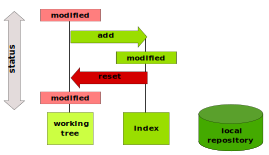
\includegraphics{diagrams/undo-staged}}
\end{frame}


\subsection{Resetting modifications}
\begin{frame}[fragile]
\subslidetitle
  After \cmd{git reset}, the modification is still there:
\begin{lstlisting}
$ (*\textcolor[HTML]{0000AA}{git status}*)
On branch master
Your branch is up-to-date with 'origin/master'.
Changes not staged for commit:
  (use "git add <file>..." to update what will be committed)
  (use "git checkout -- <file>..." to discard changes in working directory)

        (*\textcolor[HTML]{AA0000}{modified:}*)   (*\textcolor[HTML]{AA0000}{AUTHORS}*)
\end{lstlisting}

  Instead of using \cmd{git checkout} on each file, \\
  use \cmd{git reset --hard} to reset all modifications at once:
\begin{lstlisting}
$ (*\textcolor[HTML]{0000AA}{git reset --hard}*)
HEAD is now at fc92204 change title
\end{lstlisting}
\end{frame}

\subsection{Removing a file}
\begin{frame}[fragile]
\subslidetitle
  Let's first create a file and commit it:
\begin{lstlisting}
$ (*\textcolor[HTML]{0000AA}{touch test.file}*)
$ (*\textcolor[HTML]{0000AA}{git add test.file}*)
$ (*\textcolor[HTML]{0000AA}{git commit -m "adding a test file"}*)
[master 3d0539f] add test file
 1 file changed, 0 insertions(+), 0 deletions(-)
 create mode 100644 test.file
\end{lstlisting}
\end{frame}

\subsection{Removing a file}
\begin{frame}[fragile]
\subslidetitle
  The command \cmd{git rm} removes a file from the repository:
\begin{lstlisting}
$ (*\textcolor[HTML]{0000AA}{git rm test.file}*)
rm 'test.file'
$ (*\textcolor[HTML]{0000AA}{git status}*)
On branch master
Your branch is ahead of 'origin/master' by 1 commit.
  (use "git push" to publish your local commits)
Changes to be committed:
  (use "git reset HEAD <file>..." to unstage)

        (*\textcolor[HTML]{00AA00}{deleted:}*)    (*\textcolor[HTML]{00AA00}{test.file}*)
\end{lstlisting}

  Commit the staged removal of the file:
  \begin{lstlisting}
$ (*\textcolor[HTML]{0000AA}{git commit -m "we do not need the test file anymore"}*)
[master 06cb00f] remove test file
 1 file changed, 0 insertions(+), 0 deletions(-)
 delete mode 100644 test.file
\end{lstlisting}

\end{frame}

\subsection{Exercises}
\begin{frame}[fragile]
\subslidetitle
  Create a commit for each exercise below:
  \begin{exercise}
    \item Change the color of the moon to blue and\\
      commit as 'blue moon'
    \item Change the \cmd{<h1>} tag of \cmd{moon.html} to 'Git Moons' and\\
      commit as 'title in page'
    \item Add a green moon and\\
      commit as 'green moon'
  \end{exercise}

\end{frame}


\section{Work locally}
\begin{frame}[fragile]
    \slidetitle
\end{frame}

\subsection{git status}
\begin{frame}[fragile]
    \subslidetitle
\end{frame}

\subsection{git add}
\begin{frame}[fragile]
    \subslidetitle
% --patch
\end{frame}

\subsection{git commit}
\begin{frame}[fragile]
    \subslidetitle
% --amend
\end{frame}

\subsection{git reset}
\begin{frame}[fragile]
    \subslidetitle
% --hard
% --soft
% --mixed
% master@{"10 minutes ago"}
\end{frame}

\subsection{git diff}
\begin{frame}[fragile]
    \subslidetitle
% --staged
\end{frame}

\subsection{git log}
\begin{frame}[fragile]
    \subslidetitle
\end{frame}

\subsection{git grep}
\begin{frame}[fragile]
    \subslidetitle
\end{frame}

\subsection{Exercises}
\begin{frame}[fragile]
  \subslidetitle
\end{frame}

\section{Work with branches}
\begin{frame}[fragile]
    \slidetitle
In this section we will learn to use git branches.

\end{frame}

\subsection{Creating branches}
\begin{frame}[fragile]
    \subslidetitle

To create a new \textbf{foo} branch, append the branch name to the \textbf{branch} command.
\begin{lstlisting}
$ (*\textcolor[HTML]{0000AA}{git branch foo}*)
\end{lstlisting}

The \cmd{git branch} command lists you all your local branches
\begin{lstlisting}
$ (*\textcolor[HTML]{0000AA}{git branch}*)
* (*\textcolor[HTML]{00AA00}{master}*)
  foo
\end{lstlisting}

Note: the * character indicate which branch we are currently working on.
\end{frame}

\subsection{Switching to branch}
\begin{frame}[fragile]
    \subslidetitle
The \cmd{git checkout} command, is used to change the working branch
\begin{lstlisting}
$ (*\textcolor[HTML]{0000AA}{git branch}*)
* (*\textcolor[HTML]{00AA00}{master}*)
  foo
$ (*\textcolor[HTML]{0000AA}{git checkout foo}*)
Switched to branch 'foo'
$ (*\textcolor[HTML]{0000AA}{git branch}*)
  master
* (*\textcolor[HTML]{00AA00}{foo}*)
$ (*\textcolor[HTML]{0000AA}{git checkout master}*)
Switched to branch 'master'
$ (*\textcolor[HTML]{0000AA}{git checkout -b bar}*)
$ (*\textcolor[HTML]{0000AA}{git branch}*)
  master
* (*\textcolor[HTML]{00AA00}{bar}*)
\end{lstlisting}
\end{frame}

\subsection{Deleting a branch}
\begin{frame}[fragile]
    \subslidetitle
To delete an existing branch use the -d or -D flag:
\begin{lstlisting}
$ (*\textcolor[HTML]{0000AA}{git checkout master}*)
$ (*\textcolor[HTML]{0000AA}{git branch foo bar -d}*)
Deleted branch foo (was c974445).
Deleted branch bar (was 9adadac).
$ (*\textcolor[HTML]{0000AA}{git branch}*)
* (*\textcolor[HTML]{00AA00}{master}*)
\end{lstlisting}

Note: you cannot delete the branch you are currently working on.

\end{frame}

\subsection{git stash}
\begin{frame}[fragile]
    \subslidetitle
% clean, pop, 
\end{frame}

\subsection{git diff}
\begin{frame}[fragile]
    \subslidetitle
\end{frame}

\subsection{git rebase}
\begin{frame}[fragile]
    \subslidetitle
% -i
\end{frame}

\subsection{git merge}
\begin{frame}[fragile]
    \subslidetitle
\end{frame}

\subsection{git cherry}
\begin{frame}[fragile]
    \subslidetitle
\end{frame}

\subsection{Exercises}
\begin{frame}[fragile]
  \subslidetitle
\end{frame}

\section{Work with remotes}
\begin{frame}[fragile]
    \slidetitle
\end{frame}

\subsection{git remote}
\begin{frame}[fragile]
    \subslidetitle
% add
% rm/remove
% set
% update
% -v
\end{frame}

\subsection{git fetch}
\begin{frame}[fragile]
    \subslidetitle
\end{frame}

\subsection{git pull}
\begin{frame}[fragile]
    \subslidetitle
\end{frame}

\subsection{git push}
\begin{frame}[fragile]
    \subslidetitle
\end{frame}

\subsection{git origin}
\begin{frame}[fragile]
    \subslidetitle
\end{frame}

\subsection{git remote update}
\begin{frame}[fragile]
    \subslidetitle
\end{frame}

\subsection{Exercises}
\begin{frame}[fragile]
  \subslidetitle
\end{frame}

\section{Rebase vs Merge}
\begin{frame}[fragile]
    \slidetitle
\end{frame}

\subsection{Exercises}
\begin{frame}[fragile]
  \subslidetitle
\end{frame}

\section{Master merge conflict}
\begin{frame}[fragile]
    \slidetitle
\end{frame}

\subsection{Three way merge}
\begin{frame}[fragile]
    \subslidetitle
\end{frame}

\subsection{git mergetool}
\begin{frame}[fragile]
    \subslidetitle
\end{frame}


\section{Work with patches}
\begin{frame}[fragile]
    \slidetitle
\end{frame}

\subsection{git format-patch}
\begin{frame}[fragile]
    \subslidetitle
\end{frame}

\subsection{git am}
\begin{frame}[fragile]
    \subslidetitle
\end{frame}

\subsection{Exercises}
\begin{frame}[fragile]
  \subslidetitle
\end{frame}

\section{Work with pull requests}
\begin{frame}[fragile]
    \slidetitle
\end{frame}


\section{Git workflow}
\begin{frame}[fragile]
    \slidetitle
\end{frame}

\subsection{Exercises}
\begin{frame}[fragile]
  \subslidetitle
\end{frame}

\section{Git undo changes}
\begin{frame}[fragile]
    \slidetitle
\end{frame}

\subsection{git reset}
\begin{frame}[fragile]
    \subslidetitle
% --hard
% --soft
% --mixed
\end{frame}

\subsection{git checkout}
\begin{frame}[fragile]
    \subslidetitle
\end{frame}

\subsection{git reflog}
\begin{frame}[fragile]
    \subslidetitle
% combine with reset
% git reset --hard master@{"10 minutes ago"}
\end{frame}


\section{Configure git}
\begin{frame}[fragile]
  \slidetitle
  \begin{block}{Getting started with git}
    Once you have git installed you are able to configure git on 3 different levels:
    \begin{itemize}
      \option{local repository level}{path/to/repository/.git/config}
      \option{user level}{ /home/\$USER/.gitconfig }
      \option{system level}{on GNU/Linux: /etc/gitconfig}
    \end{itemize}

    The configuration file is a simple text file and can be edited with any text editor.
    Priority of git config: local, user, system.
  \end{block}
\end{frame}

\subsection{git config}
\begin{frame}[fragile]
  \subslidetitle
  The command \cmd{git config} can be used to change the global, system and local config of git.
  \begin{itemize}
      \option{git config ..}{}
      \option{git config --global ..}{}
      \option{git config --system ..}{}
  \end{itemize}
\end{frame}

\subsection{Set username and email}
\begin{frame}[fragile]
  \subslidetitle
  \vspace{1em}
  Set your name and email locally:
  \begin{itemize}
      \option{git config add user.name "My name"}{}
      \option{git config add user.email "myemail@git.ch"}{}
  \end{itemize}
  \vspace{1em}
  Or globally:
  \begin{itemize}
      \option{git config --global add user.name "My name"}{}
      \option{git config --global add user.email "myemail@git.ch"}{}
  \end{itemize}

  Extract from \bf{$\sim$/.gitconfig}
\begin{lstlisting}
[user]
  name = Andreas Schmid
  email = ikeark@gmail.com
\end{lstlisting}
\end{frame}

\subsection{Create aliases}
\begin{frame}[fragile]
  \subslidetitle

  Git allows to create aliases for commands.

  Example:

  instead of typing \bf{git status} we want to type \bf{git st}.

  Define alias:
  \begin{lstlisting}
  git config --global alias.st = status
  git config --global alias.co = checkout
  git config --global alias.ci = commit
  git config --global alias.br = branch
  \end{lstlisting}


  Extract from \bf{$\sim$/.gitconfig}
\begin{lstlisting}
[alias]
  st = status
  co = checkout
  ci = commit
  br = branch
  l = log --graph --pretty=format:'%C(yellow)%h%C(cyan)%d%Creset %s %C(white)- %an, %ar%Creset'
  ll = log --stat --abbrev-commit
\end{lstlisting}
\end{frame}

\subsection{Set mergetool}
\begin{frame}[fragile]
  \subslidetitle
\begin{lstlisting}
[merge]
  tool = kdiff3
\end{lstlisting}
\end{frame}

\subsection{Example $\sim$/.gitconfig}
\begin{frame}[fragile]
  \subslidetitle

\begin{lstlisting}
[user]
  name = Andreas Schmid
  email = ikeark@gmail.com

[core]
  pager = less -r

[color]
  diff = auto
  status = auto
  branch = auto
  grep = auto

[alias]
  st = status
  co = checkout
  ci = commit
  br = branch
  l = log --graph --pretty=format:'%C(yellow)%h%C(cyan)%d%Creset %s %C(white)- %an, %ar%Creset'
  ll = log --stat --abbrev-commit

[svn]
  addAuthorFrom = true
  useLogAuthor = true
  rmdir = true

[merge]
  tool = kdiff3

[http]
  sslVerify = false
\end{lstlisting}
\end{frame}

\subsection{Exercises}
\begin{frame}[fragile]
  \subslidetitle
    \begin{exercise}
    \item Configure git to use your name and email.
    \item Add alias \cmd{git co} for \cmd{git checkout}
    \end{exercise}
\end{frame}

\section{Extras}
\begin{frame}[fragile]
  \slidetitle
  This section covers some advanced topics:
  \begin{itemize}
    \item Cleaning workspace
    \item Working with patches
    \item Search keywords
    \item ...
  \end{itemize}
\end{frame}

\subsection{Remove untracked files}
\begin{frame}[fragile]
    \subslidetitle
  Tracking a project under git helps you to keep your workspace clean, after your compilation process generated some temporary files:

  \begin{lstlisting}
(*\textcolor[HTML]{18B2B2}{(master)}*) $ (*\textcolor[HTML]{0000AA}{touch \$(echo "compile" | hexdump | head -n1)}*)
(*\textcolor[HTML]{18B2B2}{(master)}*) $ (*\textcolor[HTML]{0000AA}{git status}*)
On branch master
...
(*\textcolor[HTML]{AA0000}{	0000000}*)
(*\textcolor[HTML]{AA0000}{	0a65}*)
(*\textcolor[HTML]{AA0000}{	6c69}*)
(*\textcolor[HTML]{AA0000}{	6f63}*)
(*\textcolor[HTML]{AA0000}{	706d}*)
...
\end{lstlisting}
  Now we would like to clean all this temporary files, using \cmd{git clean}:
  \begin{lstlisting}
(*\textcolor[HTML]{18B2B2}{(master)}*) $ (*\textcolor[HTML]{0000AA}{git git clean -df}*)
Removing 0000000
Removing 0a65
...
\end{lstlisting}

\end{frame}

\subsection{Search with git}
\begin{frame}[fragile]
  \subslidetitle
  Lost in search? It is just convenient to have \cmd{git grep}:
  \begin{lstlisting}
(*\textcolor[HTML]{18B2B2}{(master)}*) $ (*\textcolor[HTML]{0000AA}{git grep moon.js}*)
moon.html:        <script src="(*\textcolor[HTML]{AA0000}{moon.js}*)"></script>
\end{lstlisting}

  Or we can search commits that touch lines containing the keyword you are looking for using \cmd{git log --pickaxe-regexp}:
  \begin{lstlisting}
(*\textcolor[HTML]{18B2B2}{(master)}*) $ (*\textcolor[HTML]{0000AA}{git log --oneline --abbrev --pickaxe-regex "*moon*"}*)
(*\textcolor[HTML]{ae6617}{a3c399f}*) remove the blue moon
(*\textcolor[HTML]{ae6617}{93ea12c}*) change the green moon color to red
...
39719c9 initial commit
\end{lstlisting}

  Finally a option of \cmd{git branch} to search the branch a commit belongs to:
  \begin{lstlisting}
(*\textcolor[HTML]{18B2B2}{(master)}*) $ (*\textcolor[HTML]{0000AA}{git branch --contains a3c399f}*)
(*\textcolor[HTML]{00AA00}{* master}*)
\end{lstlisting}
\end{frame}

\subsection{Work with patches}
\begin{frame}[fragile]
    \subslidetitle

  Remove the blue moon:
  \begin{lstlisting}
(*\textcolor[HTML]{18B2B2}{(master)}*) $ (*\textcolor[HTML]{0000AA}{sed -i "/blue/d" moon.js}*)
(*\textcolor[HTML]{18B2B2}{(master)}*) $ (*\textcolor[HTML]{0000AA}{git commit -a -m "remove the blue moon"}*)
\end{lstlisting}

  The \cmd{git format-patch} generates patch file to be send to 3rd party collaborator, or mailing list:
  \begin{lstlisting}
(*\textcolor[HTML]{18B2B2}{(master)}*) $ (*\textcolor[HTML]{0000AA}{git format-patch -1}*)
0001-remove-the-blue-moon.patch
\end{lstlisting}

  \begin{lstlisting}
(*\textcolor[HTML]{18B2B2}{(master)}*) $ (*\textcolor[HTML]{0000AA}{cat 0001-remove-the-blue-moon.patch}*)
From 7afa035a39c2dc9648b182772eee06e3181ae24e Mon Sep 17 00:00:00 2001
From: Eric Keller <keller.eric@gmail.com>
Date: Sun, 29 Nov 2015 10:06:27 +0000
Subject: [PATCH] remove the blue moon
...
 init();
-moon( "blue" );
 moon( "white" );
...
\end{lstlisting}

\end{frame}

\subsection{Git submodules}
\begin{frame}[fragile]
  \subslidetitle
  Git offers the possibility to include other git repositories in a subdirectory of a project.
  \\
  \vspace{1em}
  The following commands deal with submodules:
  \begin{itemize}
    \item \cmd{git submodule add URL PATH}
    \item \cmd{git submodule update}
    \item \cmd{git submodule sync}
  \end{itemize}
  \vspace{1em}
  Note: the main project can commit the subdirectory and fix the commit of the submodule.
\end{frame}

\subsection{Apply a patch}
\begin{frame}[fragile]
    \subslidetitle
  First remove the last commit:
  \begin{lstlisting}
(*\textcolor[HTML]{18B2B2}{(master)}*) $ (*\textcolor[HTML]{0000AA}{git reset --hard HEAD\textasciicircum1}*)
\end{lstlisting}
  Create new no-blue branch in order to apply this patch
  \begin{lstlisting}
(*\textcolor[HTML]{18B2B2}{(master)}*) $ (*\textcolor[HTML]{0000AA}{git checkout -b no-blue}*)
Switched to a new branch 'no-blue'
\end{lstlisting}

  The \cmd{git am} command takes a list of patch to apply to the current working area:
  \begin{lstlisting}
(*\textcolor[HTML]{18B2B2}{(no-blue)}*) $ (*\textcolor[HTML]{0000AA}{git am -3 0001-remove-the-blue-moon.patch}*)
Applying: remove the blue moon
\end{lstlisting}

  Note: As well as when merging branch the \cmd{git am} could potentially end up with conflict, therefore we would like to enforce a 3way-merge with the \cmd{-3} option.

\end{frame}

\subsection{Cherrypick a commit}
\begin{frame}[fragile]
    \subslidetitle
  You are currently implementing a bugfix on a released version and should simultaneously fix it in the tip of your development, seems to be a load of work! Not if you use \cmd{git cherry-pick}:
  \begin{lstlisting}
(*\textcolor[HTML]{18B2B2}{(no-blue)}*) $ (*\textcolor[HTML]{0000AA}{git log -1 --oneline}*)
(*\textcolor[HTML]{ae6617}{1d36adc}*) remove the blue moon
\end{lstlisting}
  Change to the master branch:
  \begin{lstlisting}
(*\textcolor[HTML]{18B2B2}{(no-blue)}*) $ (*\textcolor[HTML]{0000AA}{git checkout master}*)
Switched to branch 'master'
\end{lstlisting}
  Now we try to cherry-pick the preceding commit:
  \begin{lstlisting}
(*\textcolor[HTML]{18B2B2}{(master)}*) $ (*\textcolor[HTML]{0000AA}{git cherry-pick 1d36adc}*)
[master fbd4ca8] remove the blue moon
 Date: Sun Nov 29 10:06:27 2015 +0000
 1 file changed, 1 deletion(-)
\end{lstlisting}
  Note:  The \cmd{git cherry-pick} could potencially end up with conflict.
\end{frame}

\subsection{Git aliases}
\begin{frame}[fragile]
  \subslidetitle

  Git allows to create aliases for commands.
  \\
  \vspace{1em}
  Example:
  instead of typing \cmd{git status} we want to type \cmd{git st}.
  \\
  \vspace{1em}
  Define aliases:

  \begin{lstlisting}
  git config --global alias.st = status
  git config --global alias.co = checkout
  git config --global alias.ci = commit
  git config --global alias.br = branch
  \end{lstlisting}

\end{frame}

\subsection{Example $\sim$/.gitconfig}
\begin{frame}[fragile]
  \subslidetitle

\begin{lstlisting}
[user]
  name = Tux Penguin
  email = tux@penguin

[color]
  diff = auto
  status = auto
  branch = auto
  grep = auto

[alias]
  st = status
  co = checkout
  ci = commit
  br = branch
  l = log --graph --pretty=format:'%C(yellow)%h%C(cyan)%d%Creset %s %C(white)- %an, %ar%Creset'
  ll = log --stat --abbrev-commit
\end{lstlisting}
\end{frame}



\end{document}

